
\chapter{Desenvolvimento}

Este capítulo aborda o processo de desenvolvimento do compilador proposto como um todo na linguagem Odin.
Cada etapa é encapsulado em um pacote, representado em \autoref{estrutura-de-pacotes} diferente \texttt{lexer} corresponde à tokenização da linguagem, \texttt{parser} corresponde à análise sintatica, \texttt{walker} contém funções que auxliam tanto a visualizar o resultado da analise sintatica, a AST, quando na checacgem de tipos da analise sintatixe, pois ambas dependem de fazer a transver@@@ da arvore em ordem, 
\texttt{}. A arquitetura da pipeline para o compilador é delineado na \autoref{fig-estrutura-geral-compilador}.
O repositório pode ser encontrado em \url{https://github.com/evertonse/@@@}

\begin{figure}[H]
  \caption{\label{estrutura-de-pacotes} \small Estrutura de Pacotes do Compilador.}
  \begin{center}
    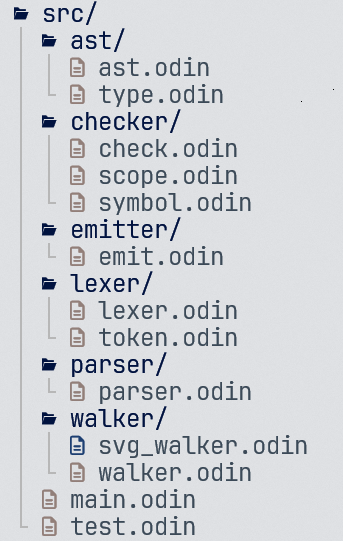
\includegraphics[scale=0.5]{./Imagens/package-structure.png}
  \end{center}
\end{figure}

\begin{figure}[H]
  \caption{\label{fig-estrutura-geral-compilador} \small Estrutura de geral da arquitetura da pipeline do Compilador.}
  \begin{center}
    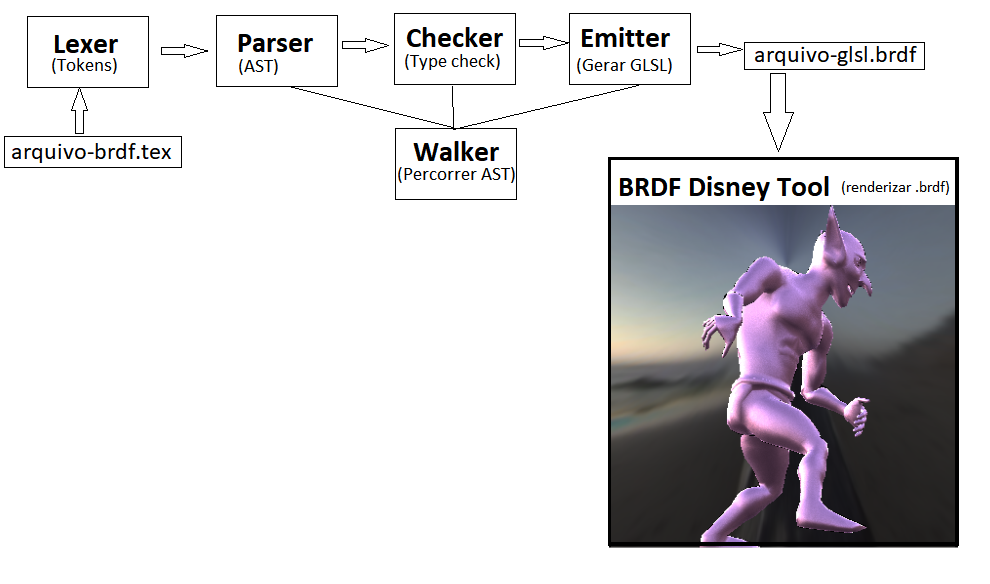
\includegraphics[scale=0.62]{./Imagens/estutura-geral-do-projeto.png}
  \end{center}
\end{figure}

Os resultados do desenvolvimento desse compilador pode ser encontrado em \autoref{resultados}.
A especificação da linguagem pode ser encontrada no \autoref{@@@}. Nesse apendice temos a gramática @@@ para tokens e gramatica que gera AST, a tabela de precedencia que é necessário para desambiguar a linguamge encontra-se em \autoref{@@@}.
Os exemplos de BRDFs mostrados no \autoref{resultados} foram usados como base para verificação da corretude da gramática durante seu desenvolvimento.

Nesta construção do compilador, foi feita análises léxica manualmente através de loops mudando o estado atual para separada a entrada, que seria um string do arquivo inteiro, para uma lista de tokens. Já a análise sintática usamos a gramática livre de contexto \autoref{@@@} para nos guiar, somado a tabela de precedencia para aplicamo o Pratt Parsing que resulta em uma AST.

% Why pratt is better:
% exemplo de como uma lingaugem um parser LALR(1) poderia fazer o encode na propria definição
%
% MultiplicativeExpr = MultiplicativeExpr * AddExpr
% AddExpr = AddExpr * Expr
%
% no prat parsing a regra de derivação é a mesma , adicionado de uma tabela
% Expr = Expr (*|+) Expr

@{Add develpment preview of wahts to come}
\subsection{Desenvolvimento}

Primeiro foi criado o analisdor lexico, um pacote inteiro para esse analisador na linguagem odin.
O trabalho desse analisdor é transform um array de caracteres que é a entrada e retonar uma sequencia de tokens.
Cada token tem um tipo ( chamado de kind em código), um valor, reservado para numeros, texto, e posição, que é usado para reportar erros.

Cada tipo (\textit{kind}) é cado pela enumeração \textbf{Token\_Kind}, essa encoda todos os possiveis tipos comomo dito @{cite previous chapter talking about the entry language}.
Esses token podem ser: comentarios gerados por uma linha que comece com \%, números, identificadores que são qualquer sequencia de caractheres que não seja palavras especiais, simbolo de igual ('='), simbolos de operadores ('\^', '*') .. bla, funções espciais ($\max$, $\sin$, $\arccos$, etc ...)


\begin{codigo}[H]
  \caption{\small } \label{}
\begin{lstlisting}
Token :: struct {
    kind: Token\_Kind,
    val: union{i64,f64},
    text: string,
    pos:  Position,
}

\end{lstlisting}
\end{codigo}

O processo de lexing feito com um loop, simulado a uma maquina de estados, que decide qual token deve ser criado em sequencia ao olhar o caractere atual e o estado.

Estados estão relacionados ao processo de identificar estados pode estar relacionados a identificar palavras.

É  adiante, por exemplo se encontrar um um '1' sabemos que é um numero, podendo ter um '.' para indicar decimal, então utilizamos 
uma subrotina para identificar esse continuar processando o "input" até o token de numeros ter sido totalmente coletado, se no meio de processar um número um caractere não esperado for encontrado, reportamos um error léxico, exemplos pode ser visto na imagem @{Mostre Imagem com Erro}
O mais simples são tokens de um caractere '\^', '*', '/', '+', '-', '?', '=', '~', '(', ')', ',', ':', '{', '}', '\_', cara um tem um proposito especifico na analise lexica. Na etapa lexica nos preopados apenas em separar nos tokens de maneira cega ao seu significado.


Todo identificador, especial ou não é processado da mesma maneira, é verificado se o caractere atual é um letra ou um '\\', isso indica o começo 
de um identificador. Depois de de

A gramatica dos tokens é regular e será representada abaixio:


Vale ressaltar que nesse moment é criado uma tabela que mapeia cada numero de linha à um string dessa mesma linha, para reportar error, printando a linha do problema mais a linha anterior e posterior para.
Tem um token que é especial que indica o começo de um ambiente `\\begin{equation}`, qualquer comentario antes de apaerecer esse token é ignorado, isso é para poder dar como entrada ao compilador um documento inteir ocontendo begin document e ainda funciojnar



\subsection{Analise Semantica}

\subsubsection{Tabela de Symbolos}
Symbolos podem ser declarados fora de ordem, ciramos um grafo de dependencias e fazemos um orednação topologica de dependencia.
Isso é póis, ao detectar analisa um certo symbolo queremos dizer se está usando simbolos não definidos, para isso precisamos definifir todos os simbolos glocais que estão no escopo visivel à todos, isso incluisimbolos pre-definidos pela linguagem, (ver tabela @{tabela de simbolos predefinidos}, para isso precisamos primeiro primeiro coletar todos esses e analisar priomeiros oq que dependen de ninguem, e medida que tão
. Também pode ocorrer dependecia circular sem reoslução e nesse caso reportamos um erro, nesse caso precisamos. @{true? ciruclar dependency?}

\subsubsection{Inferencia de Tipos}

\subsection{SVG da arvore abstrata com inferencia de tipos}
Para identificar possiveis erros de ordenação algumas medidas foram feitas para auxiliar, como a geração de uma imagem da 
em SVG da arvore sintatica, já com inferencia de tipos


